% answers.tex —— 2017 年·上海普通高考卷 · 参考答案与详细解析片段
% 由 tools/generate_projects.py 依来源总账自 2017/2017_数学真题_上海_试题.md + 2017/2017_数学真题_上海_解析正文.md + 2017/2017_数学真题_上海_答案要点.md 生成，勿手改（改源 MD 后重跑）


\begin{gktip}
固定来源 PDF 只有题面，没有答案、解析或评分材料。以下为编者独立推导并逐题复算的非官方解析；来源文件的发布者、出版物、版次、原始来源链及官方身份仍未核实。Q20（3）保留题面给出的向量关系，由这些关系推得点 $Q$，没有增补题设条件。
\end{gktip}

\begin{answer}
\gksolhead{1}{}

\textbf{题目}：

已知集合 $A=\{1,2,3,4\}$，集合 $B=\{3,4,5\}$，则 $A\cap B=\underline{\qquad}$。

\Needspace{4\baselineskip}
\textbf{解析}

两个集合的公共元素是 $3$ 和 $4$，故 $A\cap B=\{3,4\}$。

\gkanswer{答案：$\{3,4\}$}

\end{answer}
\begin{answer}
\gksolhead{2}{}

\textbf{题目}：

若排列数 $P_6^m=6\times5\times4$，则 $m=\underline{\qquad}$。

\Needspace{4\baselineskip}
\textbf{解析}

$P_6^m$ 是由 $6$ 起连续取 $m$ 个因子的乘积。$6\times5\times4$ 恰有三个因子，因此 $m=3$。

\gkanswer{答案：$3$}

\end{answer}
\begin{answer}
\gksolhead{3}{}

\textbf{题目}：

不等式 $\dfrac{x-1}{x}>1$ 的解集为 $\underline{\qquad}$。

\Needspace{4\baselineskip}
\textbf{解析}

移项得 $\dfrac{x-1}{x}-1=-\dfrac1x>0$，所以 $x<0$，解集为 $(-\infty,0)$。

\gkanswer{答案：$(-\infty,0)$}

\end{answer}
\begin{answer}
\gksolhead{4}{}

\textbf{题目}：

已知球的体积为 $36\pi$，则该球主视图的面积等于 $\underline{\qquad}$。

\Needspace{4\baselineskip}
\textbf{解析}

由 $\dfrac43\pi r^3=36\pi$ 得 $r=3$。球的主视图是半径为 $3$ 的圆，其面积为 $9\pi$。

\gkanswer{答案：$9\pi$}

\end{answer}
\begin{answer}
\gksolhead{5}{}

\textbf{题目}：

已知复数 $z$ 满足 $z+\dfrac{3}{z}=0$，则 $|z|=\underline{\qquad}$。

\Needspace{4\baselineskip}
\textbf{解析}

$z+\dfrac3z=0$ 且 $z\ne0$，故 $z^2=-3$。于是 $|z|^2=|z^2|=3$，所以 $|z|=\sqrt3$。

\gkanswer{答案：$\sqrt3$}

\end{answer}
\begin{answer}
\gksolhead{6}{}

\textbf{题目}：

设双曲线 $\dfrac{x^2}{9}-\dfrac{y^2}{b^2}=1\ (b>0)$ 的焦点为 $F_1,F_2$，$P$ 为该双曲线上的一点，若 $|PF_1|=5$，则 $|PF_2|=\underline{\qquad}$。

\Needspace{4\baselineskip}
\textbf{解析}

双曲线上一点到两焦点的距离差的绝对值等于实轴长 $2a=6$。若 $|PF_1|=5$，则另一焦距只能与 $5$ 相差 $6$；距离为负的候选值 $-1$ 不可能，故 $|PF_2|=11$。

\gkanswer{答案：$11$}

\end{answer}
\begin{answer}
\gksolhead{7}{}

\textbf{题目}：

如图，以长方体 $ABCD-A_1B_1C_1D_1$ 的顶点 $D$ 为坐标原点，过 $D$ 的三条棱所在的直线为坐标轴，建立空间直角坐标系。若 $\overrightarrow{DB_1}$ 的坐标为 $(4,3,2)$，则 $\overrightarrow{AC_1}$ 的坐标是 $\underline{\qquad}$。
\nopagebreak[4]
\begin{center}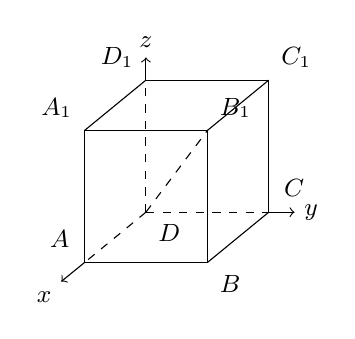
\begin{tikzpicture}[x=0.78cm,y=0.78cm,every node/.style={font=\small}]
  % Source-faithful cuboid topology; projection lengths are schematic.
  \coordinate (D)  at (0,0);
  \coordinate (A)  at (-1.0,-0.82);
  \coordinate (C)  at (2.0,0);
  \coordinate (B)  at (1.0,-0.82);
  \coordinate (D1) at (0,2.15);
  \coordinate (A1) at (-1.0,1.33);
  \coordinate (C1) at (2.0,2.15);
  \coordinate (B1) at (1.0,1.33);

  % Visible cuboid edges.
  \draw (A) -- (B);
  \draw (B) -- (C);
  \draw (A) -- (A1);
  \draw (B) -- (B1);
  \draw (C) -- (C1);
  \draw (A1) -- (B1);
  \draw (B1) -- (C1);
  \draw (C1) -- (D1);
  \draw (D1) -- (A1);

  % Hidden cuboid edges along the three coordinate axes.
  \draw[dashed] (D) -- (A);
  \draw[dashed] (D) -- (C);
  \draw[dashed] (D) -- (D1);

  % The source also shows the vector DB_1 as a dashed diagonal.
  \draw[dashed] (D) -- (B1);

  % Positive coordinate directions continue beyond the corresponding vertices.
  \draw[->] (A) -- (-1.38,-1.13) node[below left] {$x$};
  \draw[->] (C) -- (2.42,0) node[right] {$y$};
  \draw[->] (D1) -- (0,2.52) node[above] {$z$};

  \node[below right=1pt] at (D) {$D$};
  \node[above left=2pt] at (A) {$A$};
  \node[below right=1pt] at (B) {$B$};
  \node[above right=2pt] at (C) {$C$};
  \node[above left=1pt] at (D1) {$D_1$};
  \node[above left=1pt] at (A1) {$A_1$};
  \node[above right=1pt] at (B1) {$B_1$};
  \node[above right=1pt] at (C1) {$C_1$};
\end{tikzpicture}
\end{center}
\nopagebreak[4]
\Needspace{4\baselineskip}
\textbf{解析}

设 $D$ 到 $A,C,D_1$ 三个方向的坐标轴依次为 $x,y,z$ 轴。由 $\overrightarrow{DB_1}=(4,3,2)$，可写 $A=(4,0,0)$、$C_1=(0,3,2)$。因此 $\overrightarrow{AC_1}=C_1-A=(-4,3,2)$。

\gkanswer{答案：$(-4,3,2)$}

\end{answer}
\begin{answer}
\gksolhead{8}{}

\textbf{题目}：

\Needspace{5\baselineskip}
定义在 $(0,+\infty)$ 上的函数 $y=f(x)$ 的反函数为 $y=f^{-1}(x)$。若
\nopagebreak[4]
\[
g(x)=
\begin{cases}
3^x-1,&x\leqslant0,\\
f(x),&x>0,
\end{cases}
\]
为奇函数，则 $f^{-1}(x)=2$ 的解为 $\underline{\qquad}$。

\Needspace{4\baselineskip}
\textbf{解析}

对 $x>0$，奇函数条件给出 $f(x)=-g(-x)=-(3^{-x}-1)=1-3^{-x}$。方程 $f^{-1}(x)=2$ 等价于 $x=f(2)$，故 $x=1-3^{-2}=\dfrac89$。

\gkanswer{答案：$\dfrac89$}

\end{answer}
\begin{answer}
\gksolhead{9}{}

\textbf{题目}：

已知四个函数：① $y=-x$，② $y=-\dfrac1x$，③ $y=x^3$，④ $y=x^{\frac12}$。从中任选 2 个，则事件“所选 2 个函数的图象有且仅有一个公共点”的概率为 $\underline{\qquad}$。

\Needspace{4\baselineskip}
\textbf{解析}

从四个函数中选两种共有 $\binom42=6$ 种。逐对求交点：①与②有两个，①与③有一个，①与④有一个，②与③没有，②与④没有，③与④有两个。恰有一个公共点的组合为两种，所求概率为 $\dfrac26=\dfrac13$。

\gkanswer{答案：$\dfrac13$}

\end{answer}
\begin{answer}
\gksolhead{10}{}

\textbf{题目}：

\Needspace{5\baselineskip}
已知数列 $\{a_n\}$ 和 $\{b_n\}$，其中 $a_n=n^2$，$n\in\mathbb N^*$；$\{b_n\}$ 的项是互不相等的正整数。若对于任意 $n\in\mathbb N^*$，$\{b_n\}$ 的第 $a_n$ 项都等于 $\{a_n\}$ 的第 $b_n$ 项，则
\nopagebreak[4]
\[
\dfrac{\lg(b_1b_4b_9b_{16})}{\lg(b_1b_2b_3b_4)}=\underline{\qquad}
\]
。

\Needspace{4\baselineskip}
\textbf{解析}

题设给出 $b_{n^2}=a_{b_n}=b_n^2$。取 $n=1$ 得正整数 $b_1=b_1^2$，故 $b_1=1$；再取 $n=2,3,4$，得 $b_4=b_2^2$、$b_9=b_3^2$、$b_{16}=b_4^2=b_2^4$。于是分子为 $\lg(b_2^6b_3^2)$，分母为 $\lg(b_2^3b_3)$。因 $b_2$ 是与 $b_1=1$ 不同的正整数，分母非零，原比值为 $2$。

\gkanswer{答案：$2$}

\end{answer}
\begin{answer}
\gksolhead{11}{}

\textbf{题目}：

\Needspace{5\baselineskip}
设 $\alpha_1,\alpha_2\in\mathbb R$，且
\nopagebreak[4]
\[
\dfrac{1}{2+\sin\alpha_1}+\dfrac{1}{2+\sin(2\alpha_2)}=2
\]
，
则 $|10\pi-\alpha_1-\alpha_2|$ 的最小值等于 $\underline{\qquad}$。

\Needspace{4\baselineskip}
\textbf{解析}

因为 $-1\leqslant\sin t\leqslant1$，每个倒数项都不超过 $1$。两项之和为 $2$，只能两项都等于 $1$，所以 $\sin\alpha_1=-1$ 且 $\sin(2\alpha_2)=-1$。因此 $\alpha_1=\dfrac{3\pi}{2}+2k\pi$、$\alpha_2=\dfrac{3\pi}{4}+l\pi$，其中 $k,l\in\mathbb Z$。于是 $\alpha_1+\alpha_2=\dfrac{9\pi}{4}+m\pi$，$m\in\mathbb Z$；它与 $10\pi$ 的距离最小为 $\dfrac\pi4$。

\gkanswer{答案：$\dfrac\pi4$}

\end{answer}
\begin{answer}
\gksolhead{12}{}

\textbf{题目}：

如图，用 35 个单位正方形拼成一个矩形，点 $P_1,P_2,P_3,P_4$ 以及四个标记为“▲”的点在正方形的顶点处。设集合 $\Omega=\{P_1,P_2,P_3,P_4\}$，点 $P\in\Omega$，过 $P$ 作直线 $l_P$，使得不在 $l_P$ 上的“▲”的点分布在 $l_P$ 的两侧。用 $D_1(l_P)$ 和 $D_2(l_P)$ 分别表示 $l_P$ 一侧和另一侧的“▲”的点到 $l_P$ 的距离之和。若过 $P$ 的直线 $l_P$ 中有且只有一条满足 $D_1(l_P)=D_2(l_P)$，则 $\Omega$ 中所有这样的 $P$ 为 $\underline{\qquad}$。
\nopagebreak[4]
\begin{center}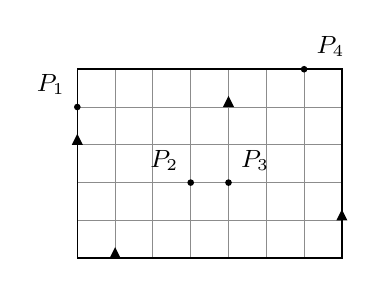
\begin{tikzpicture}[x=0.48cm,y=0.48cm,every node/.style={font=\small}]
  % Seven columns by five rows of unit squares; coordinates are only for redraw.
  \draw[step=1,black!45,line width=0.35pt] (0,0) grid (7,5);
  \draw[line width=0.55pt] (0,0) rectangle (7,5);

  % Marked P-points from the source.
  \fill (0,4) circle (1.2pt);
  \node[above left=1pt] at (0,4) {$P_1$};
  \fill (3,2) circle (1.2pt);
  \node[above left=1pt] at (3,2) {$P_2$};
  \fill (4,2) circle (1.2pt);
  \node[above right=1pt] at (4,2) {$P_3$};
  \fill (6,5) circle (1.2pt);
  \node[above right=1pt] at (6,5) {$P_4$};

  % The four solid triangles occupy the source lattice vertices.
  \fill (1,0) ++(-2pt,0) -- ++(2pt,4pt) -- ++(2pt,-4pt) -- cycle;
  \fill (0,3) ++(-2pt,0) -- ++(2pt,4pt) -- ++(2pt,-4pt) -- cycle;
  \fill (4,4) ++(-2pt,0) -- ++(2pt,4pt) -- ++(2pt,-4pt) -- cycle;
  \fill (7,1) ++(-2pt,0) -- ++(2pt,4pt) -- ++(2pt,-4pt) -- cycle;
\end{tikzpicture}
\end{center}
\nopagebreak[4]
\Needspace{4\baselineskip}
\textbf{解析}

\Needspace{5\baselineskip}
按图中格点取四个“▲”点坐标为 $(1,0),(7,1),(0,3),(4,4)$，其坐标和为 $(12,8)$。若过 $P=(p,q)$ 的直线法向量为 $\mathbf n$，四点到直线的有向距离之和与
\nopagebreak[4]
\[
\mathbf n\cdot\bigl((12,8)-4(p,q)\bigr)
\]
成正比。若括号中的向量非零，平衡条件确定唯一法向方向；还需核对直线两侧均有标记点。逐点计算：

\begin{itemize}
\item $P_1=(0,4)$ 时，唯一候选直线为 $2x+3y=12$，四个标记点位于直线两侧且均不在直线上，距离和相等。
\item $P_2=(3,2)$ 时，$(12,8)-4P_2=(0,0)$，每条过 $P_2$ 的直线都满足有向距离和为零；可取的分割方向不止一条，故不符合“有且只有一条”。
\item $P_3=(4,2)$ 时，唯一候选直线为 $y=2$，标记点分居两侧且没有标记点在线上。
\item $P_4=(6,5)$ 时，唯一候选直线为 $x-y=1$；点 $(1,0)$ 在直线上，其余三个点分居两侧，两侧距离和均为 $5/\sqrt2$。题面只要求不在线上的标记点分居两侧，因此该直线符合条件。
\end{itemize}

故所求为 $\{P_1,P_3,P_4\}$。

\gkanswer{答案：$\{P_1,P_3,P_4\}$}

\end{answer}
\begin{answer}
\gksolhead{13}{}

\textbf{题目}：

\Needspace{5\baselineskip}
关于 $x,y$ 的二元一次方程组
\nopagebreak[4]
\[
\begin{cases}
x+5y=0,\\
2x+3y=4,
\end{cases}
\]
的系数行列式 $D$ 为（　）。

（A）$\begin{vmatrix}0&5\\4&3\end{vmatrix}$　（B）$\begin{vmatrix}1&0\\2&4\end{vmatrix}$　（C）$\begin{vmatrix}1&5\\2&3\end{vmatrix}$　（D）$\begin{vmatrix}6&0\\5&4\end{vmatrix}$

\Needspace{4\baselineskip}
\textbf{解析}

系数行列式按未知数 $x,y$ 的系数排列为 $D=\begin{vmatrix}1&5\\2&3\end{vmatrix}$，对应选项 C。

\gkanswer{答案：C}

\end{answer}
\begin{answer}
\gksolhead{14}{}

\textbf{题目}：

在数列 $\{a_n\}$ 中，$a_n=\left(-\dfrac12\right)^n$，$n\in\mathbb N^*$，则 $\displaystyle\lim_{n\to\infty}a_n$（　）。

（A）等于 $-\dfrac12$　（B）等于 $0$　（C）等于 $\dfrac12$　（D）不存在

\Needspace{4\baselineskip}
\textbf{解析}

因为 $\left|(-\dfrac12)^n\right|=(\dfrac12)^n\to0$，故 $a_n\to0$，选项 B 正确。

\gkanswer{答案：B}

\end{answer}
\begin{answer}
\gksolhead{15}{}

\textbf{题目}：

已知 $a\text{、}b\text{、}c$ 为实常数，数列 $\{x_n\}$ 的通项 $x_n=an^2+bn+c$，$n\in\mathbb N^*$，则“存在 $k\in\mathbb N^*$，使得 $x_{100+k},x_{200+k},x_{300+k}$ 成等差数列”的一个必要条件是（　）。

（A）$a\geqslant0$　（B）$b\leqslant0$　（C）$c=0$　（D）$a-2b+c=0$

\Needspace{4\baselineskip}
\textbf{解析}

三项成等差数列的条件是 $x_{100+k}-2x_{200+k}+x_{300+k}=0$。代入 $x_n=an^2+bn+c$ 后，一次项和常数项相消，左侧等于 $2a\cdot100^2$，所以必须 $a=0$。因此选项 A 的 $a\geqslant0$ 是必要条件。

\gkanswer{答案：A}

\end{answer}
\begin{answer}
\gksolhead{16}{}

\textbf{题目}：

\Needspace{5\baselineskip}
在平面直角坐标系 $xOy$ 中，已知椭圆 $C_1:\dfrac{x^2}{36}+\dfrac{y^2}{4}=1$ 和 $C_2:x^2+\dfrac{y^2}{9}=1$。$P$ 为 $C_1$ 上的动点，$Q$ 为 $C_2$ 上的动点，$w$ 是 $\overrightarrow{OP}\cdot\overrightarrow{OQ}$ 的最大值。记
\nopagebreak[4]
\[
\Omega=\{(P,Q)\mid P\text{ 在 }C_1\text{ 上，}Q\text{ 在 }C_2\text{ 上，且 }\overrightarrow{OP}\cdot\overrightarrow{OQ}=w\},
\]
则 $\Omega$ 中（　）。

（A）元素个数为 2　（B）元素个数为 4　（C）元素个数为 8　（D）含有无穷个元素

\Needspace{4\baselineskip}
\textbf{解析}

\Needspace{5\baselineskip}
令 $P=(6\cos t,2\sin t)$、$Q=(\cos u,3\sin u)$，则
\nopagebreak[4]
\[
\overrightarrow{OP}\cdot\overrightarrow{OQ}=6\cos t\cos u+6\sin t\sin u=6\cos(t-u)\leqslant6.
\]
当 $t=u$ 时取最大值 $6$；任意 $t$ 都得到一个不同的有序点对 $(P,Q)$，故达到最大值的点对有无穷多个，选项 D 正确。

\gkanswer{答案：D}

\end{answer}
\begin{answer}
\gksolhead{17}{}

\textbf{题目}：

如图，直三棱柱 $ABC-A_1B_1C_1$ 的底面为直角三角形，两直角边 $AB$ 和 $AC$ 的长分别为 4 和 2，侧棱 $AA_1$ 的长为 5。

（1） 求三棱柱 $ABC-A_1B_1C_1$ 的体积；

（2） 设 $M$ 是 $BC$ 中点，求直线 $A_1M$ 与平面 $ABC$ 所成角的大小。
\nopagebreak[4]
\begin{center}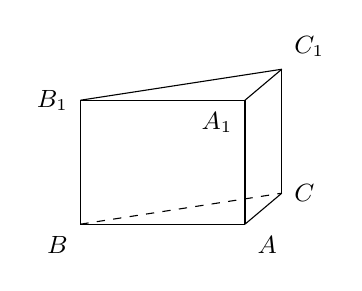
\begin{tikzpicture}[x=0.82cm,y=0.82cm,every node/.style={font=\small}]
  % Source-faithful triangular-prism topology; projection lengths are schematic.
  \coordinate (B)  at (0,0);
  \coordinate (A)  at (2.55,0);
  \coordinate (C)  at (3.12,0.48);
  \coordinate (B1) at (0,1.92);
  \coordinate (A1) at (2.55,1.92);
  \coordinate (C1) at (3.12,2.40);

  % Solid edges shown in the source diagram.
  \draw (B) -- (A);
  \draw (A) -- (C);
  \draw (A) -- (A1);
  \draw (B) -- (B1);
  \draw (C) -- (C1);
  \draw (B1) -- (A1);
  \draw (A1) -- (C1);
  \draw (B1) -- (C1);

  % The hidden base edge BC is dashed in the source.
  \draw[dashed] (B) -- (C);

  \node[below left=1pt] at (B) {$B$};
  \node[below right=1pt] at (A) {$A$};
  \node[right=1pt] at (C) {$C$};
  \node[left=1pt] at (B1) {$B_1$};
  \node[below left=1pt] at (A1) {$A_1$};
  \node[above right=1pt] at (C1) {$C_1$};
\end{tikzpicture}
\end{center}
\nopagebreak[4]
\Needspace{4\baselineskip}
\textbf{解析}

\gksubpart{(1)}

底面直角三角形面积为 $\dfrac12\cdot4\cdot2=4$，棱柱高为 $5$，体积为 $4\cdot5=20$。

\gksubpart{(2)}

$BC=\sqrt{4^2+2^2}=2\sqrt5$。直角三角形斜边中线长为斜边的一半，所以 $AM=\sqrt5$。直线 $A_1M$ 在平面 $ABC$ 上的射影为 $AM$，故所成角 $\theta$ 满足 $\tan\theta=AA_1/AM=5/\sqrt5=\sqrt5$，即 $\theta=\arctan\sqrt5$。

\gkanswer{答案（1）：$20$}

\gkanswer{答案（2）：$\arctan\sqrt5$}

\end{answer}
\begin{answer}
\gksolhead{18}{}

\textbf{题目}：

已知函数 $f(x)=\cos^2x-\sin^2x+\dfrac12$，$x\in(0,\pi)$。

（1） 求 $f(x)$ 的单调递增区间；

（2） 设 $\triangle ABC$ 为锐角三角形，角 $A$ 所对边 $a=\sqrt{19}$，角 $B$ 所对边 $b=5$。若 $f(A)=0$，求 $\triangle ABC$ 的面积。

\Needspace{4\baselineskip}
\textbf{解析}

\gksubpart{(1)}

$f(x)=\cos2x+\dfrac12$，$f'(x)=-2\sin2x$。在给定定义域 $(0,\pi)$ 内，$f'(x)>0$ 的区间为 $(\dfrac\pi2,\pi)$；函数在 $x=\dfrac\pi2$ 连续，故最大单调递增区间写为 $[\dfrac\pi2,\pi)$。

\gksubpart{(2)}

\Needspace{5\baselineskip}
$f(A)=0$ 给出 $\cos2A=-\dfrac12$。因 $A$ 为锐角，得 $A=\dfrac\pi3$。由正弦定理，
\nopagebreak[4]
\[
\sin B=\frac{b\sin A}{a}=\frac{5\sqrt3}{2\sqrt{19}},\qquad \cos B=\frac1{2\sqrt{19}},
\]
\Needspace{5\baselineskip}
其中余弦取正是因为 $B$ 为锐角。于是
\nopagebreak[4]
\[
\sin C=\sin(A+B)=\sin A\cos B+\cos A\sin B=\frac{3\sqrt3}{2\sqrt{19}}.
\]
三角形面积为 $\dfrac12 ab\sin C=\dfrac{15\sqrt3}{4}$。

\gkanswer{答案（1）：$[\dfrac\pi2,\pi)$}

\gkanswer{答案（2）：$\dfrac{15\sqrt3}{4}$}

\end{answer}
\begin{answer}
\gksolhead{19}{}

\textbf{题目}：

\Needspace{5\baselineskip}
根据预测，某地第 $n$（$n\in\mathbb N^*$）个月共享单车的投放量和损失量分别为 $a_n$ 和 $b_n$（单位：辆），其中
\nopagebreak[4]
\[
a_n=
\begin{cases}
5n^4+15,&1\leqslant n\leqslant3,\\
-10n+470,&n\geqslant4,
\end{cases}
\qquad b_n=n+5
\]
，
第 $n$ 个月底的共享单车的保有量是前 $n$ 个月的累计投放量与累计损失量的差。

（1） 求该地区第 4 个月底的共享单车的保有量；

（2） 已知该地共享单车停放点第 $n$ 个月底的单车容纳量 $S_n=-4(n-46)^2+8800$（单位：辆）。设在某月底，共享单车保有量达到最大，问该保有量是否超出了此时停放点的单车容纳量？

\Needspace{4\baselineskip}
\textbf{解析}

\gksubpart{(1)}

前四个月投放量依次为 $20,95,420,430$ 辆，前四个月损失量之和为 $6+7+8+9=30$ 辆。因此第 4 个月底保有量为 $20+95+420+430-30=935$ 辆。

\gksubpart{(2)}

第 $n\geqslant4$ 个月的保有量净增量为 $a_n-b_n=(-10n+470)-(n+5)=465-11n$。该增量在 $n\leqslant42$ 时为正，在 $n\geqslant43$ 时为负；前三个月净增量也均为正，所以保有量在第 42 个月底达到最大。

\Needspace{5\baselineskip}
前 42 个月总投放量为
\nopagebreak[4]
\[
20+95+420+\sum_{n=4}^{42}(-10n+470)=535+9360=9895,
\]
\Needspace{5\baselineskip}
总损失量为 $\sum_{n=1}^{42}(n+5)=903+210=1113$，最大保有量为 $9895-1113=8782$ 辆。容量
\nopagebreak[4]
\[
S_{42}=-4(42-46)^2+8800=8736,
\]
故超出 $8782-8736=46$ 辆。

\gkanswer{答案（1）：$935$ 辆}

\gkanswer{答案（2）：保有量在第 $42$ 个月底达到最大，为 $8782$ 辆；该月容量为 $8736$ 辆，超出 $46$ 辆。}

\end{answer}
\begin{answer}
\gksolhead{20}{}

\textbf{题目}：

在平面直角坐标系 $xOy$ 中，已知椭圆 $\Gamma:\dfrac{x^2}{4}+y^2=1$，$A$ 为 $\Gamma$ 的上顶点，$P$ 为 $\Gamma$ 上异于上、下顶点的动点，$M$ 为 $x$ 轴正半轴上的动点。

（1） 若 $P$ 在第一象限，且 $|OP|=\sqrt2$，求 $P$ 的坐标；

（2） 设 $P\left(\dfrac85,\dfrac35\right)$，若以 $A\text{、}P\text{、}M$ 为顶点的三角形是直角三角形，求 $M$ 的横坐标；

（3） 若 $|MA|=|MP|$，直线 $AQ$ 与 $\Gamma$ 交于另一点 $C$，且 $\overrightarrow{AQ}=2\overrightarrow{AC}$，$\overrightarrow{PQ}=4\overrightarrow{PM}$，求直线 $AQ$ 的方程。

\begin{gktip}
\textbf{转录边界}：Q20（3）按源文保留关于点 $Q$ 的两组向量关系。独立解析由这些关系与其余条件确定 $Q$，未增补题设条件。
\end{gktip}

\Needspace{4\baselineskip}
\textbf{解析}

\gksubpart{(1)}

联立椭圆方程 $x^2/4+y^2=1$ 与 $|OP|^2=x^2+y^2=2$，相减得 $3x^2/4=1$，所以 $x^2=4/3$、$y^2=2/3$。由 $P$ 在第一象限，得 $P=(\dfrac{2\sqrt3}{3},\dfrac{\sqrt6}{3})$。

\gksubpart{(2)}

设 $M=(t,0)$，其中 $t>0$。直角不可能在 $A$ 点，因为 $\overrightarrow{AP}\cdot\overrightarrow{AM}=(8t+2)/5>0$。直角在 $P$ 点时，$\overrightarrow{PA}\cdot\overrightarrow{PM}=0$，化简得 $t=29/20$。直角在 $M$ 点时，$\overrightarrow{MA}\cdot\overrightarrow{MP}=0$，即 $t^2-\dfrac85t+\dfrac35=0$，解得 $t=1$ 或 $t=3/5$。三值均为正，故均符合题意。

\gksubpart{(3)}

设 $P=(x,y)$、$M=(t,0)$、$A=(0,1)$。由 $|MA|=|MP|$ 得 $2tx=x^2+y^2-1$。又 $P$ 在椭圆上，$x^2/4+y^2=1$，故 $x^2+y^2-1=3x^2/4$。题设 $P$ 异于上下顶点，$x\ne0$；并且 $t>0$，所以 $x>0$ 且 $t=3x/8$。

\Needspace{5\baselineskip}
向量条件给出 $Q=4M-3P$，而 $\overrightarrow{AQ}=2\overrightarrow{AC}$ 给出 $C=(A+Q)/2$。代入 $t=3x/8$，得
\nopagebreak[4]
\[
C=(-3x/4,(1-3y)/2).
\]
\Needspace{5\baselineskip}
由于 $C$ 在椭圆上，$x^2/4+y^2=1$ 导出 $27y^2-24y-3=0$，即 $(y-1)(9y+1)=0$。$y=1$ 会使 $x=0$，与 $P$ 异于上下顶点矛盾；因此 $y=-1/9$，再由 $x>0$ 得 $x=8\sqrt5/9$。于是
\nopagebreak[4]
\[
M=(\sqrt5/3,0),\quad C=(-2\sqrt5/3,2/3),\quad Q=(-4\sqrt5/3,1/3).
\]
直线 $AQ$ 的斜率为 $1/(2\sqrt5)=\sqrt5/10$，故方程为 $y=1+\dfrac{\sqrt5}{10}x$。

\gkanswer{答案（1）：$(\dfrac{2\sqrt3}{3},\dfrac{\sqrt6}{3})$}

\gkanswer{答案（2）：$\dfrac{29}{20},\ 1,\ \dfrac35$}

\gkanswer{答案（3）：$y=1+\dfrac{\sqrt5}{10}x$}

\end{answer}
\begin{answer}
\gksolhead{21}{}

\textbf{题目}：

设定义在 $\mathbb R$ 上的函数 $f(x)$ 满足：对于任意的 $x_1,x_2\in\mathbb R$，当 $x_1<x_2$ 时，都有 $f(x_1)\leqslant f(x_2)$。

（1） 若 $f(x)=ax^3+1$，求 $a$ 的取值范围；

（2） 若 $f(x)$ 是周期函数，证明：$f(x)$ 是常值函数；

（3） 设 $f(x)$ 恒大于零。$g(x)$ 是定义在 $\mathbb R$ 上的、恒大于零的周期函数，$M$ 是 $g(x)$ 的最大值。函数 $h(x)=f(x)g(x)$。证明：“$h(x)$ 是周期函数”的充要条件是“$f(x)$ 是常值函数”。

\Needspace{4\baselineskip}
\textbf{解析}

\gksubpart{(1)}

$x^3$ 在实数范围内严格递增，故 $a\geqslant0$ 时 $ax^3+1$ 单调不减；若 $a<0$，该函数严格递减，不可能单调不减。因此 $a\geqslant0$。

\gksubpart{(2)}

\Needspace{5\baselineskip}
设 $T>0$ 是 $f$ 的一个周期。任取 $x<y$，取正整数 $n$ 使 $x+nT>y$。由单调性和周期性，
\nopagebreak[4]
\[
f(x)\leqslant f(y)\leqslant f(x+nT)=f(x),
\]
所以 $f(x)=f(y)$。任意两点函数值相同，故 $f$ 为常值函数。

\gksubpart{(3)}

若 $f$ 为常值函数，则 $h=fg$ 具有 $g$ 的周期。

\Needspace{5\baselineskip}
反过来，设 $h$ 有正周期 $T$，并取 $x_0$ 使 $g(x_0)=M$。对任意正整数 $n$，由 $f$ 不减、$g\leqslant M$ 及 $h$ 的周期性，
\nopagebreak[4]
\[
f(x_0)M=h(x_0)=h(x_0-nT)=f(x_0-nT)g(x_0-nT)\leqslant f(x_0)M.
\]
因 $f>0$ 且 $g\leqslant M$，等号迫使 $f(x_0-nT)=f(x_0)$。再由单调性可知 $f(x)=f(x_0)$ 对所有 $x\leqslant x_0$ 成立。

\Needspace{5\baselineskip}
$g$ 的最大值沿其任一正周期反复出现，因此可取任意大的最大值点 $y\geqslant x_0$。选正整数 $m$ 使 $y-mT\leqslant x_0$。利用 $h$ 的周期性、$f(y-mT)=f(x_0)$ 和 $g\leqslant M$，得
\nopagebreak[4]
\[
f(y)M=h(y)=h(y-mT)\leqslant f(x_0)M,
\]
所以 $f(y)\leqslant f(x_0)$。另一方面 $y\geqslant x_0$ 且 $f$ 不减，故 $f(y)\geqslant f(x_0)$，于是 $f(y)=f(x_0)$。对任意 $x\geqslant x_0$，取最大值点 $y\geqslant x$，单调性给出 $f(x_0)\leqslant f(x)\leqslant f(y)=f(x_0)$，故 $f(x)=f(x_0)$。因此 $f$ 在全实数范围为常值函数。

\gkanswer{答案（1）：$a\geqslant0$}

\gkanswer{答案（2）：见解析版}

\gkanswer{答案（3）：见解析版}

\end{answer}